\chapter{Market impact models}
\label{chap:market_impact_models}
A market impact model explains how prices react to trades, or more broadly, to orders placed in the market. If we consider $m_n$ the midprice at time $n$:
\begin{align*}
	& \Delta m_n \equiv m_{n+1} - m_n = \\
	&F(\epsilon_n, \epsilon_{n-1},\ldots;v_n,v_{n-1},\ldots;\Omega_n,\Omega_{n-1},\ldots;\Delta m_{n-1},\Delta m_{n-2},\ldots; x_n \ldots) + \eta_n
\end{align*}
where:
\begin{itemize}
	\item $\epsilon_n = \pm 1$ is the sign of traders
	\item $v_n$ is the volume of the trade(s)
	\item $\Omega_n$ is the state of the order book
	\item $x_n$ are other covariates
	\item $\eta_n$ is noise term
\end{itemize}
The dynamics of the (mid)-price is deterministically given by the flow of all the orders (e.g. limit orders, market orders, and cancellations).
\section{Response function and lagged return variance}
We introduce two diagnostics to test (and calibrate) empirical market impact models:
\begin{itemize}
	\item The \textbf{response function} is defined as:
	\[
	\mathcal{R}\mathnormal{(l)} \equiv \expected{\epsilon_n \cdot (m_{n+l} - m_n)}
	\]
	and measures the expected price shift between $n$ and $n+l$ conditioned to the sign of the trade at time $n$
	\item The \textbf{lagged return variance} is defined as:
	\[
	\mathcal{V}(l) \equiv \expected{(m_{n+l} -m_n)^2}
	\]
	it is the variance of the price on a time scale $l$.
\end{itemize}
Plotting $\mathcal{V}/l$ versus $l$, we obtain signature plot, which is expected to tend to a constant if $l \to \infty$ (long term volatility)
\begin{center}
	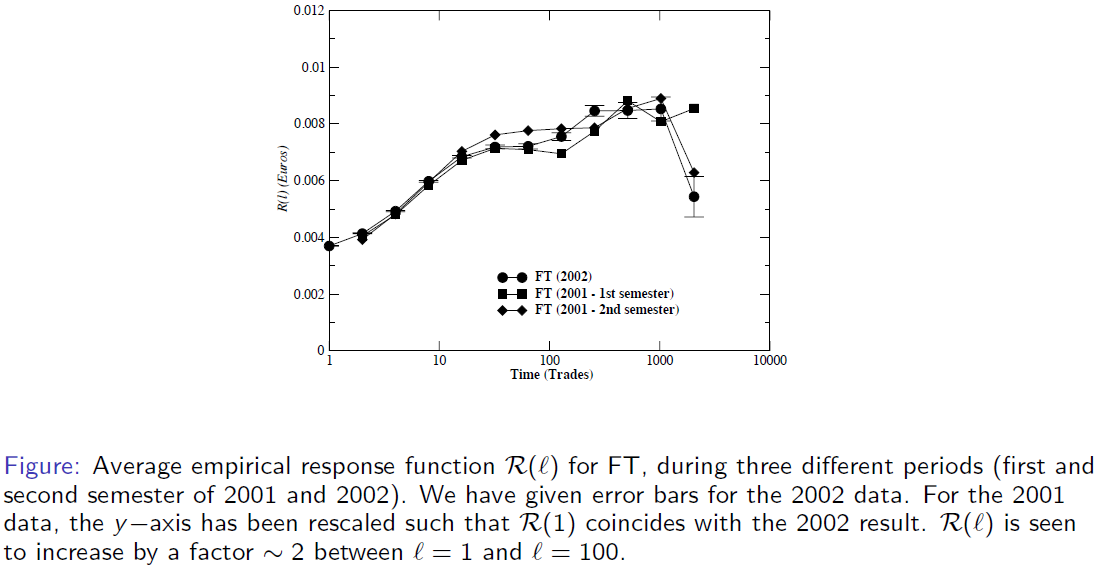
\includegraphics[width=0.7\textwidth]{picture/(6)empirical_response.png}
\end{center}
\subsection{A firs fixed permanent impact model}
\begin{mysetting}[Fixed permanent impact model]
	\begin{itemize}
		\item $r_n$ is the midquote price change between just before the $n$th trade and just before the $n + 1$th trade.
		\item Immediate impact, $\expected{r_n | \epsilon_n v_n}$, is non zero and can be written as $\expected{r_n | \epsilon_n v_n} = \epsilon f(v)$, where $f$ is a function that grows with $v$
		\item Impact of a transaction is permanent, like in usual random walks, and the equation for the midquote price $m_n$ at time $n$ is:
		\[
		r_n = m_{n+1} - m_n = \epsilon_n f(v_n;\Omega_n) + \eta_n
		\]
		where $\eta_n$ is random term describing price changes not directlu attrivuted to trading itself (for example news). We assume $\eta_n$ is indepndent on the order glow and we set $\expected{\eta} = 0$ and $\expected{\eta^2} = \Sigma^2$
	\end{itemize}
\end{mysetting}
\begin{mysetting}
	\begin{itemize}
				\item We have incorporated the idea that the impact of a trade can be influenced by the current state of the order book $\Omega_n$. This inclusion is justified on general principles: when a market order with a volume $v_n$ interacts with a substantial queue of limit orders, it typically exerts only a minimal impact on the price. Conversely, one can anticipate a strong correlation between the state of the order book, $\Omega_n$, and the magnitude of incoming market orders: larger volumes of limit orders tend to attract larger market orders.
	\end{itemize}
\end{mysetting}
We can express the midquote price as:
\[
m_n = \sum_{k<n} \epsilon_k f(v_k; \Omega_k) + \sum_{k<n} \eta_k
\]
This equation show a non-decaying nature of the impact, $\epsilon_k \partial m_n/ \partial v_k$ ($k <n$) does not decay as $n-k$ grows.\\
Lagged impact function $\mathcal{R}(l)$ and lagged return variance $\mathcal{V}(l)$ is:
\[
\mathcal{R}(l) = \expected{f} \qquad \mathcal{V}(l) = \left(\expected{f^2} + \Sigma^2\right)l
\]
constant price impact and pure price diffusion, close to what is indeed observed empirically on small tick, liquid contracts.\\
At the same time, the autocovariance of price returns:
\[
\expected{r_nr_{n + \tau}} \propto \expected{\epsilon_n \epsilon_{n+\tau]}}\sim \tau^{-\gamma}
\]
with $\gamma$ small. That means that price returns are strongly autocorrelated in time. But this would violate market efficiency hypothesis, in fact price returns would be easy predictable.\\
So empirically observed long memory of order flow is incompatible with the random walk model if price are efficient.
\begin{myquote}
	How can the market be statistically efficient (i.e. unpredictable) in the presence of an autocorrelated order flow?
\end{myquote}
\section{Madhavan, Richardson and Roomans (MRR) model}
\begin{mysetting}[MRR model]
	\begin{itemize}
		\item all trades have the same volume $v_n = v$ and the $\epsilon_n$’s are generated by a Markov process with correlation $\rho$, thus $\expected{\epsilon_n|\epsilon_{n-1} = \rho \epsilon_{n-1}}$
		\item correlations decay exponentially fast, i.e. $C(l) = \expected{\epsilon_i \epsilon_{i+l}} = \rho^l$ which does not conform to reality.
	\end{itemize}
\end{mysetting}
\begin{mysetting}
\begin{itemize}
	\item The MRR model postulates that the mid-point $m_n$ evolves only because of unpredictable external shocks (or news) and because of the surprise component in the order flow. This postulate of course automatically removes any predictability in the price returns and ensures efficiency:
	\[
	m_{n+1} - m_n = \theta[\epsilon_n - \rho \epsilon_{n-1}] + \eta_n
	\]
	where $\eta$ iss shock component, $\theta$ measure the size of trade impact
\end{itemize}
\end{mysetting}
We can rewrite price return as:
\[
m_{n+l} - m_n = \sum_{j=n}^{n+l-1} \eta_j + \theta \sum_{j =n}^{n+l-1} [\epsilon_j - \rho \epsilon_{j-1}]
\]
The full impact function is found to be constant, equal to:
\[
\mathcal{R}(l) = \theta(1 - \rho^2), \qquad \forall l
\]
We can introduce the function $G(l)$ thet measure the influence of a single trade at time $n-l$ on the mid-point at time $n$:
\begin{equation}
m_n = \sum_{j = -\infty}^{n-1}\eta_j + \sum_{j = -\infty}^{n-1} G (n-j-1)\eta_j
\label{mid_point_G_MRR}
\end{equation}
in this way we can impose $G(l=0) = \theta$ and $G(l\geq 1) = \theta(1-\rho)$: a part of $\theta \rho$ of impact instantaneously decays to zero after first trade, whereas the rest of the impact is permanent.\\
The volatility in this model can be written as:
\[
\mathcal{V}(l) = [ \theta^2(1-  \rho^2) +\Sigma^2]l
\]
\begin{mysetting}[The MRR model with bid-ask spread]
	\begin{itemize}
		\item The original MRR model assumes that it is the ‘true’ fundamental price $p_n$, rather
		than the midpoint $m_n$, which is impacted by the surprise in order flow, and hence:
		\[
		p_{n+1} - p_n = \eta_n + \theta[\epsilon_n - \rho \epsilon_{n-1}]
		\]
		\item Market Makers cannt guess the surprise of the next trade, so bid and ask price are given by:
		\[
		a_n = p_n + \theta[1- \rho \epsilon_{n-1}] + \phi \qquad b_n = p_n + \theta[- 1- \rho \epsilon_{n-1}] - \phi 
		\]
		where $\phi$ is extra compension due to shock component risk.
	\end{itemize}
\end{mysetting}

\begin{mysetting}
	\begin{itemize}
		\item The midpoint $m \equiv = (a+b)/2$ immediately before the $n$th trade is:
		\[
		m_n = p_n - \theta \rho \epsilon_{n-1}
		\]
	whereas the spread is given by $S = a-b = 2(\theta + \phi)$
	\end{itemize}
\end{mysetting}
If we neglecting $\phi$ for arbitrary correlations between signs:
\[
m_{n+l} - m_n = \sum_{j=n}^{n+l-1} \eta_n + \theta \sum_{j =n }^{n + l-1} \left\{\epsilon_j - \expected{\epsilon_{j+1}}_j\right\}
\]
Than, the impact function is:
\[
\mathcal{R}(l) = \theta[1 - C(l)]
\]
So that $\mathcal{R}(\infty) = \theta = S/2$, the long term profit of market makers is zero (Spread and impact are two sides of the same coin).\\
Long time impact is enhanced compared to the short term impact by factor:
\[
\lambda \equiv \frac{\mathcal{R} (\infty)}{\mathcal{R}(1)} = \frac{1}{1 -C(1)} > 1
\]
If $\phi \neq 0$:
\[
S = 2(\theta + \phi) = 2(\mathcal{R}(\infty) + \phi) = 2\lambda \mathcal{R}(1) + 2\phi
\]
where $\lambda = (1- \rho)^{-1}$.\\
We can write mid-point volatility on scale $l$:
\[
\sigma^2_l = \frac{1}{l} \expected{(m_{l+i} - m_i)^2}
\]
and it is the sum of trade induced volatility $\theta^2(1-\rho)^2$ and a news induced volatility $\Sigma^2$:
\begin{align*}
	& \sigma_1^2 = \expected{(m_{n+1} -m+n)^2} = \Sigma^2 + \theta^2(1-\rho)^2\\
	& \sigma^2_\infty = \Sigma^2 + \theta^2 (1-\rho)^2 \left(1 + 2 \frac{\rho}{1-\rho}\right) = \Sigma^2 + \theta^2(1 -\rho^2) \geq \sigma_1^2 
\end{align*}
The MRR model leads to two simple relations between spread, impact and volatility per trade:
\[
S = 2\lambda\mathcal{R}(1) + 2\phi \qquad \sigma_1^2 = \mathcal(1)^2 + \Sigma^2
\]
With empirical data, it fits quite well.\\
Some general comments:
\begin{itemize}
	\item 
	The linear relationship between the spread and volatility per trade is not anticipated to remain valid when considering the volatility per unit of time $\sigma$. This is because the latter incorporates an additional factor, which is both stock-dependent and time-dependent, namely the trading frequency denoted as $f$ which can be expressed as: 
	\[
	\sigma = \sigma_1 \sqrt{f}
	\]
	\item There are two complementary economic interpretations of the relation $\sigma_1 \sim S$ in small tick markets
	\begin{itemize}
		\item Given that the typical liquidity available in the order book is relatively limited, market orders often capture a significant portion of the volume at the best available price. Additionally, it's observed that the size of the "gap" above the ask or below the bid is roughly comparable in magnitude to the bid-ask spread itself. Consequently, both the market impact and the volatility per trade are expected to be of the same order of magnitude as the stock price, denoted as "S," as has been empirically observed.
		\item This relationship can also be interpreted inversely, where when the volatility per trade is high, the risk associated with placing limit orders increases. Consequently, the spread tends to widen until it becomes advantageous to use limit orders.
	\end{itemize}
\end{itemize}
Let us continue the discussion on long-term memory. We have said that long term memory of trades is a priori paradoxical and hints towards a non trivial property of financial markets, which can be called long-term resilience.\\
Using equation \ref{mid_point_G_MRR} and assuming that single trade impact is lag independent $G(l) =G$ and that volume fluctuations can be neglected, mid price variance can be computed as:
\[
\mathcal{V}(l)\equiv \expected{(m_{n+l} - m_n)^2} = \underbrace{[ \Sigma^2 + G^2]}_{\text{diffusive process}}l + 2G \sum_{j =1}^{l} (l-j) C(j)
\]
When $\gamma <1$, the second therm of RHS can be approximated ($l \ell 1$) by $2c_0Gl^{2-\gamma}/(1-\gamma)(2-\gamma)$, which grows faster than the first term.\\
The price would super diffuse, at long times, trend with a volatility diverging with the lag $l$. This phenomena does not occur, in fact the market reacts to trade correlations so as to prevent the occurrence of such trends.
\section{Transient impact model (TIM)}
\begin{mydefinition}[Propagator model (Bouchaud 2004)]
\begin{equation}
	m_t = \sum_{t'<t} [G(t-t')\epsilon_{t'} + \eta_{t'}] + m_{-\infty}
\end{equation}
The term $G(t-t'$) avoid super-diffusivity.\\
In differential form, setting $r_t = m_{t+1}-m_t$:
\begin{equation}
	r_t = G(1)\epsilon_t + \sum_{t'<t} \mathcal{G} (t-t)\epsilon_{t'} + \eta_t \qquad \mathcal{G}(l) \equiv G(l+1)-G(l)
\end{equation}
where $G(l\leq 0) \equiv 0$
\end{mydefinition}
In this setting, past order flow affects future returns, and we do not require efficiency (martingale assumption).\\
The lagged price variance can be computed as:
\[
\mathcal{V}(l) = \sum_{0\leq j <l} G^2(l-j) + \sum_{j>0} [ G(l+j) - G(j)]^2 + 2 \Delta(l) + \Sigma^2l
\]
where $\Delta(l)$ is the correlation induced contribution:
\begin{align*}
	\Delta(l) = & \sum_{0\leq j < k <l} G(l-j)G(l-k)C(k-j)\\
	& + \sum_{0<j<k} [G(l+j) - G(j)][G(l+k) -G(k)]C(k-j) \\
	& + \sum_{0\leq j <l}\sum_{k>0} G(l-j) [G(l+k) - G(k)]C(k+j)
\end{align*}
Assuming $G(l)$ decays at large $l$  as $G(l)\sim \Gamma_0l^{-\beta}$, if $\beta,\gamma <1$, than:
\[
\Delta(l) \sim \Gamma_0^2c_oI(\gamma,\beta)l^{2-2\beta-\gamma}
\]
where $I>0$ is a numerical integral.
General comments on this model:
\begin{itemize}
	\item if single trade impact does not decay $(\beta = 0)$, we have superdiffusive result.
	\item As impact decays faster, superdiffusion is reduced.
	\item At a critical value $\beta_c  = (1-\gamma)/2$, grows linearly with $l$ and contributes to the long term value of the volatility
	\item If $\beta > \beta_c$, $\Delta(l)$ grows sublinear with $l$, impact enhances high frequency value compared to long term $\Sigma^2$
	\item Long range correlation in order flow grows not induce long term correlations nor anticorrelations in price returns iff the impact of single trades is transiet ($\beta >0$) but itself non-summable ($\beta <1$)
\end{itemize}
\begin{mydefinition}[Continuous time version of the TIM (Gatheral 2010)]
Let us consider an unperturbed martingale dynamics of the price:
\[
dS^0_t = \sigma_tdW_t
\]
where $\sigma_t$ is volatility and $W_t$ is Wiener process.\\
When trading $dX_t = \dot{X}_tdt$ shares in the interval $[]t, t+dt]$, the price follows this eqution:
\end{mydefinition}
\begin{mydefinition}
	\begin{equation}
		S_t^X = S_0 + \int_{0}^{T} f(\dot{X}_s)G(t-s)ds + \int_{0}^t \sigma_sdW_s
	\end{equation}
	$f(\dot{X}_s)$ is velocity function and $G(t-s)$ evaluate how the pass influence the future
\end{mydefinition}
If $f(x) = kx$, the settinf is the same as TIM.\\
The avarage impact function $\mathcal{R}(l)$ of model is:
\[
\mathcal{R}(l) = G(l) + \sum_{0<j<l}G(l-j)C(j) + \sum_{j>0} [G(l+j) - G(j)]C(j)
\]
So that $C(n)$ and $\mathcal{R}(l)$ are measurable quantity, from them we can evaluate $G(l)$.\\
An alternative method less sensitive to boundary effects is using response function $\mathcal{S}(l) = \expected{r_{r+l}\cdots \epsilon_t}$  and $C(l)$:
\[
\mathcal{S}(l) = \sum_{n\geq 0} \mathcal{G}(n)C(n-l)
\]
whose solution represents the values of the kernel $\mathcal{G}(l)$.\\
Exist a relationship beween response and impact function:
\[
\mathcal{R}(l) = \sum_{0\leq i<l}\mathcal{S}(i)
\]
Asymptotically, when $G(l)$ decays as $\Gamma_0l^{-\beta}$, if $\beta + \gamma <1$:
\[
\mathcal{R}(l) \sim l^{1-\beta-\gamma}
\] 
\begin{itemize}
	\item $\beta<\beta_c$: $\mathcal{R}(l)$ diverges to $+ \infty$ for large $l$
	\item  $\beta>\beta_c$: $\mathcal{R}(l)$ diverges to $- \infty$
This means that when the decay of single trade impact is too fast, the accumulation of meatn reverting effects leads to a negative long term average impact.
\item $\beta = \beta_c$ $\mathcal{R}(l) \to \mathcal{R}(\infty)$, the decay of single trade impact precisely offsets the positive correlation of the trades
\end{itemize}
